\chapter{Construcción de un agujero negro y el enigma del horizonte cercano}

\lectureoverview{Construiremos un agujero negro a partir de tres elementos: el diagrama causal del espacio-tiempo plano, el diagrama de Schwarzschild y el teorema de Birkhoff para una capa esférica. La construcción revela que un horizonte de sucesos es una frontera global y que puede comenzar en una región que todavía es localmente plana. Luego pasaremos de la geometría causal a la entropía y la temperatura de Hawking. Un termómetro sostenido cerca del horizonte se calienta sin límite, mientras que un observador en caída libre no espera ninguna catástrofe local. El argumento final pregunta qué puede demostrar realmente un experimento exterior sin producir la perturbación que pretende detectar.}

\section{Un agujero negro a la temperatura del espacio vacío}

Se suponía que había tarea: construir un agujero negro y llevarlo a clase para mostrarlo. Nadie tenía uno que pudiera exhibir, pero un cálculo encontrado con Wolfram nos proporcionó un problema inicial más accesible. ¿Qué radio y qué masa tendría que tener un agujero negro para que su temperatura de Hawking fuera cercana a la \(3\,\mathrm{K}\) temperatura del fondo cósmico de microondas?

\begin{classroomqa}
\audiencequestion{¿Qué se calculó en el sitio web?\lecturetimestamp{00:00:39}}
\lecturerresponse{El radio de un agujero negro cuya temperatura es de aproximadamente \(3\,\mathrm{K}\). No se busca un cálculo preciso, sino estimar la escala física.}
\end{classroomqa}

Un agujero así tendría momentáneamente la misma temperatura que su entorno, pero el equilibrio sería inestable. Un agujero negro de Schwarzschild tiene capacidad calorífica negativa. Si se calienta un poco más que el baño térmico, emite radiación, pierde masa y se calienta aún más. Si se enfría un poco por debajo de su temperatura, absorbe energía, gana masa y se enfría todavía más.\editorialnote{Este es el argumento preciso de estabilidad que subyace a la formulación deliberadamente aproximada empleada en clase. Un baño térmico canónico no puede mantener en equilibrio estable un agujero negro de Schwarzschild aislado.}

La estimación comienza con la longitud de onda característica de la radiación a \(3\,\mathrm{K}\).

\begin{classroomqa}
\audiencequestion{¿Qué longitud de onda corresponde a una radiación de unos tres kelvin?\lecturetimestamp{00:02:03}}
\lecturerresponse{En la sala se propusieron un centímetro, \(21\) centímetros e incluso \(10\) metros antes de llegar al intervalo de las microondas. Para el argumento bastaba con una respuesta aproximada del orden de un centímetro, lo bastante pequeña para hacer los chistes sobre un horno de microondas y una caja de pan.}
\end{classroomqa}

El cuanto de Hawking típico tiene una longitud de onda comparable, salvo factores numéricos, con el radio de Schwarzschild:
\begin{equation}
\lambda_{\mathrm{H}}\sim R_s,
\qquad
R_s=\frac{2GM}{c^2}.
\label{eq:l05-scale}
\end{equation}
Al tomar el valor usado en clase, \(\lambda_{\mathrm H}\sim1\,\mathrm{cm}\), se obtiene \(R_s\sim1\,\mathrm{cm}\). Como un agujero negro de masa solar tiene un radio de unos pocos kilómetros y \(R_s\) es proporcional a \(M\), la masa correspondiente es aproximadamente
\begin{equation}
M\sim10^{-5}M_\odot,
\label{eq:l05-rough-mass}
\end{equation}
una escala planetaria. Por eso, en la clase se llega a una estimación similar a la masa de la Tierra.

\begin{classroomqa}
\audiencequestion{¿Concuerda con el resultado numérico de Wolfram?\lecturetimestamp{00:05:53}}
\lecturerresponse{El resultado indicado estaba más cerca de la masa de la Luna. Parecía pequeña en comparación con la estimación aproximada, pero cualquiera de las dos respuestas permite llegar al punto buscado: no es un objeto que uno pueda llevar en el bolsillo.}
\end{classroomqa}

Al conservar las constantes se explica la discrepancia. A partir de
\begin{equation}
T_H=\frac{\hbar c}{4\pi k_B R_s},
\end{equation}
se obtiene, para \(T_H=3\,\mathrm{K}\),
\begin{equation}
R_s\simeq6.1\times10^{-5}\,\mathrm{m},
\qquad
M\simeq4.1\times10^{22}\,\mathrm{kg}.
\label{eq:l05-three-kelvin}
\end{equation}
una masa lunar, no terrestre. La longitud de onda de las microondas, el factor \(4\pi\) y la elección de qué longitud de onda del cuerpo negro se considera típica explican la diferencia entre la estimación rápida y el valor numérico.\editorialnote{La ecuación~\eqref{eq:l05-three-kelvin} restituye los factores numéricos omitidos en la estimación dimensional de la clase. Se conserva la estimación porque ese fue el razonamiento seguido en clase.}

El cálculo ya ha cumplido su propósito. Ahora queremos construir un agujero negro, tanto matemáticamente como en la imaginación. Las ecuaciones de campo completas son demasiado difíciles para lo que necesitamos aquí. Los diagramas nos darán los hechos básicos.

\section{El primer elemento: el espacio-tiempo plano}

Usamos coordenadas polares centradas en un observador y omitimos los ángulos. Las coordenadas reducidas son \((t,r)\), con \(r\geq0\). Un punto de este diagrama reducido no es un punto del espacio-tiempo cuatridimensional; salvo cuando \(r=0\), representa una esfera completa \(S^2\).

Los rayos de luz radiales se desplazan a \(45^\circ\). Un rayo entrante llega al origen, y uno saliente parte de allí en la otra dirección nula. El semiplano infinito se puede comprimir en una cuña de Penrose finita mediante una transformación conforme. La transformación no es única. Lo esencial es que lleva el infinito a una frontera finita y que las direcciones nulas radiales siguen formando un ángulo de \(45^\circ\). En palabras usadas en la pizarra, aplastamos el diagrama.

\begin{figure}[htbp]
\centering
\includegraphics[width=0.68\textwidth]{lecture_05_figure_02.png}
\caption{Mitad superior del espacio de Minkowski radial compactificado. El borde vertical es \(r=0\), mientras que las familias de curvas se apiñan hacia el infinito compactificado.}
\lectureframe{00:11:41.560}
\end{figure}

\begin{figure}[htbp]
\centering
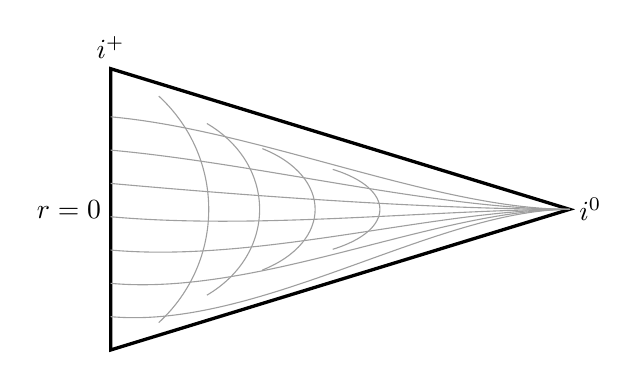
\begin{tikzpicture}[scale=0.94]
\coordinate (O) at (0,0);
\coordinate (P) at (0,3.8);
\coordinate (I) at (6.2,1.9);
\draw[very thick] (O)--(P)--(I)--cycle;
\foreach \y in {0.45,0.90,1.35,1.80,2.25,2.70,3.15} {
  \draw[gray!75] (0,\y) .. controls (2.0,\y-0.18) and (4.4,1.9) .. (I);
}
\draw[gray!75] (0.65,0.37) .. controls (1.55,1.20) and (1.55,2.60) .. (0.65,3.43);
\draw[gray!75] (1.30,0.74) .. controls (2.25,1.30) and (2.25,2.50) .. (1.30,3.06);
\draw[gray!75] (2.05,1.08) .. controls (3.00,1.46) and (3.00,2.34) .. (2.05,2.72);
\draw[gray!75] (3.00,1.36) .. controls (3.85,1.62) and (3.85,2.18) .. (3.00,2.44);
\node[left] at (0,1.9) {\(r=0\)};
\node[above] at (P) {\(i^+\)};
\node[right] at (I) {\(i^0\)};
\end{tikzpicture}
\caption{Una versión limpia de la cuña superior. Las curvas son familias cualitativas de valores constantes de \(r\) y de \(t\), no una cuadrícula exacta de coordenadas.}
\label{fig:l05-flat-wedge}
\end{figure}

Las líneas de universo con \(r\) constante, verticales antes de la compactificación, se curvan y se acumulan cerca del infinito temporal futuro. Las secciones de \(t\) constante también se apiñan hacia el infinito espacial. Este apiñamiento es un efecto de las coordenadas, no una compresión física de la materia.

La regla de \(45^\circ\) se aplica directamente a la luz radial. Un rayo con momento angular puede no pasar por el origen: alcanza una distancia mínima no nula y luego vuelve hacia afuera. Lejos del origen, su movimiento proyectado parece casi radial; solo cerca de la distancia mínima se aprecia la curvatura de la trayectoria reducida \((t,r)\). Así concluye el primer elemento.

\section{El segundo elemento: Schwarzschild eterno}

La solución de Schwarzschild maximalmente extendida tiene dos regiones exteriores en forma de rombo, una región de agujero negro futuro y una región de agujero blanco pasado. Sus fronteras onduladas superior e inferior son las singularidades futura y pasada. En breve descartaremos gran parte de esta estructura para describir un agujero negro formado por colapso, pero la región exterior derecha ordinaria es justo la que necesitamos.

\begin{figure}[htbp]
\centering
\includegraphics[width=0.72\textwidth]{lecture_05_figure_03.png}
\caption{Diagrama de Schwarzschild eterno, con la región exterior ordinaria y su cuadrícula esquemática de coordenadas a la derecha.}
\lectureframe{00:16:55.975}
\end{figure}

\begin{figure}[htbp]
\centering
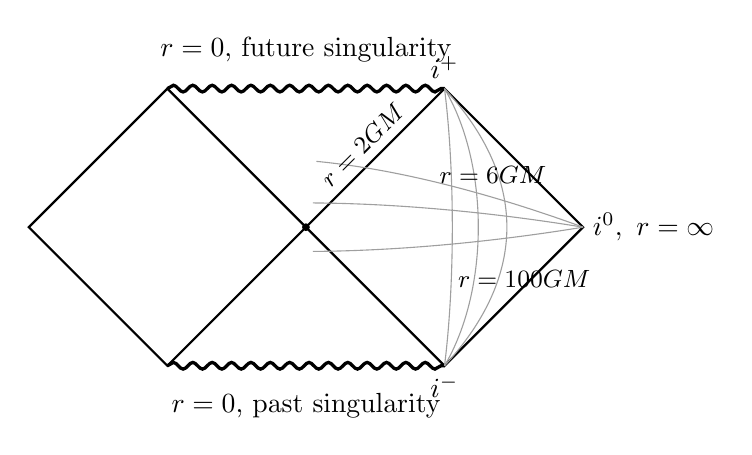
\begin{tikzpicture}[scale=0.88]
\coordinate (C) at (0,0);
\coordinate (TL) at (-2.0,2.0);
\coordinate (L) at (-4.0,0);
\coordinate (BL) at (-2.0,-2.0);
\coordinate (TR) at (2.0,2.0);
\coordinate (R) at (4.0,0);
\coordinate (BR) at (2.0,-2.0);
\draw[thick] (C)--(TL)--(L)--(BL)--(C);
\draw[thick] (C)--(TR)--(R)--(BR)--(C);
\draw[very thick,decorate,decoration={snake,amplitude=1.2pt,segment length=7pt}] (TL)--(TR);
\draw[very thick,decorate,decoration={snake,amplitude=1.2pt,segment length=7pt}] (BL)--(BR);
\draw[gray!75] (TR) .. controls (2.15,0.8) and (2.15,-0.8) .. (BR);
\draw[gray!75] (TR) .. controls (2.65,0.9) and (2.65,-0.9) .. (BR);
\draw[gray!75] (TR) .. controls (3.20,0.7) and (3.20,-0.7) .. (BR);
\draw[gray!75] (0.15,0.95) .. controls (1.5,0.82) and (2.9,0.40) .. (R);
\draw[gray!75] (0.10,0.35) .. controls (1.5,0.34) and (2.9,0.18) .. (R);
\draw[gray!75] (0.10,-0.35) .. controls (1.5,-0.34) and (2.9,-0.18) .. (R);
\fill (C) circle (1.6pt);
\node[above] at (TR) {\(i^+\)};
\node[below] at (BR) {\(i^-\)};
\node[right] at (R) {\(i^0,\ r=\infty\)};
\node[above] at (0,2.25) {\(r=0\), future singularity};
\node[below] at (0,-2.25) {\(r=0\), past singularity};
\node[rotate=45,above,font=\small] at (1.0,1.0) {\(r=2GM\)};
\node[font=\small] at (2.70,0.75) {\(r=6GM\)};
\node[font=\small] at (3.15,-0.75) {\(r=100GM\)};
\end{tikzpicture}
\caption{La región exterior derecha se parece a la cuña plana a radios grandes. Su borde nulo interior es \(r=2GM\) cuando \(c=1\); los otros radios indicados son ejemplos esquemáticos.}
\label{fig:l05-eternal-schwarzschild}
\end{figure}

Lejos del agujero, la región exterior se parece cada vez más al espacio plano compactificado. Líneas como \(r=6GM\) y \(r=100GM\) se aproximan al comportamiento de líneas de universo ordinarias de radio constante. La frontera interior de la región exterior está en
\begin{equation}
r=2GM
\end{equation}
en unidades \(c=1\).

Cerca del centro, la comparación con el espacio plano deja de ser válida. Un rayo radial en el espacio de Minkowski llega a \(r=0\) y vuelve a emerger por el lado físico opuesto. Un rayo dirigido hacia el futuro dentro de Schwarzschild no rebota: termina en la singularidad espacial en \(r=0\). La construcción por colapso debe preservar esta diferencia causal.

\section{El teorema que permite unir los elementos}

El ingrediente que faltaba aparece primero en la gravedad newtoniana. Para una distribución de masa esféricamente simétrica, la ley de Gauss da
\begin{equation}
\oint\mathbf g\cdot d\mathbf A=-4\pi G M_{\mathrm{enc}},
\end{equation}
y, por tanto,
\begin{equation}
\mathbf g(r)=-\frac{G M_{\mathrm{enc}}(r)}{r^2}\,\hat{\mathbf r}.
\label{eq:l05-shell-theorem}
\end{equation}
La materia situada fuera de la esfera de radio \(r\) no contribuye al campo neto en su interior. Para una capa hueca de masa total \(M\),
\begin{equation}
\mathbf g=
\begin{cases}
0, & r<R_{\mathrm{shell}},\\[3pt]
-\dfrac{GM}{r^2}\hat{\mathbf r}, & r>R_{\mathrm{shell}}.
\end{cases}
\end{equation}

El teorema de Birkhoff es su equivalente relativista. Toda región de vacío esféricamente simétrica es localmente una región de Schwarzschild con un parámetro de masa constante. El interior vacío de una capa esférica tiene parámetro de masa nulo y es localmente minkowskiano; el exterior tiene parámetro de masa \(M\) y es de Schwarzschild:
\begin{equation}
\begin{aligned}
M_{\mathrm{enc}}&=0 && \text{inside the shell},\\
M_{\mathrm{enc}}&=M && \text{outside the shell}.
\end{aligned}
\label{eq:l05-birkhoff}
\end{equation}
El enunciado sigue siendo útil aunque la capa se mueva, porque las regiones de vacío a ambos lados siguen siendo esféricamente simétricas.

\editorialnote{Que el interior sea plano es un enunciado local. Una capa estática puede cambiar la normalización de la coordenada temporal interior aunque la curvatura allí sea nula. Para una capa móvil o nula, hay que empalmar las dos métricas de vacío a través de la capa; esta construcción idealizada es un empalme de capa delgada, estrechamente relacionado con la geometría de Vaidya entrante. Ninguna de estas precisiones cambia el argumento causal de recortar y pegar que empleamos aquí.}

Para imaginarlo en el laboratorio, pensemos en una esfera densamente cubierta de láseres sincronizados, como los de una gran instalación de confinamiento inercial, todos disparados hacia adentro a la vez. En la idealización no hay ningún dispositivo: solo una capa perfectamente esférica de luz. La capa transporta energía \(E\), de modo que el parámetro de masa exterior es
\begin{equation}
M=\frac{E}{c^2},
\end{equation}
o simplemente \(E=M\) en unidades naturales. Como la capa se desplaza a la velocidad de la luz, en el diagrama reducido es una línea nula entrante. Cada punto de esa línea representa un frente de onda esférico completo, no la trayectoria de un único fotón.

\section{Empalme del espacio-tiempo de colapso}

Partimos del espacio-tiempo plano y dibujamos la capa nula entrante. La región interior a la capa es correcta: el teorema de Birkhoff dice que es plana. La exterior es incorrecta, porque su geometría de Schwarzschild debe reflejar ya la masa total de la capa.

Ahora dibujamos la misma capa en el diagrama de Schwarzschild eterno. Allí es correcta la región exterior a la capa. El agujero blanco, la segunda región exterior y la parte inadecuada del interior del agujero negro no corresponden a un colapso que empieza en un espacio vacío ordinario, así que los borramos.

\begin{figure}[htbp]
\centering
\includegraphics[width=0.72\textwidth]{lecture_05_figure_05.png}
\caption{La capa nula, en rojo, trazada sobre el diagrama de Schwarzschild mientras se aísla la parte correcta de la región exterior.}
\lectureframe{00:32:00.000}
\end{figure}

En el tramo plano, la capa llega a \(r=0\). En el tramo de Schwarzschild, llega al comienzo de la singularidad futura. Es el mismo punto final. Al pegar el interior plano a la región exterior de Schwarzschild a lo largo de la capa se obtiene el espacio-tiempo más sencillo de formación de un agujero negro.

\begin{classroomqa}
\audiencequestion{En el punto de empalme de arriba a la izquierda, ¿coincide realmente el punto final en el espacio plano con el punto del lado de Schwarzschild?\lecturetimestamp{00:34:50}}
\lecturerresponse{Sí. La capa en el espacio plano se contrae hasta \(r=0\), y la singularidad de Schwarzschild también está en \(r=0\). Los dos puntos identificados tienen el mismo significado geométrico: la esfera bidimensional se ha contraído hasta tener tamaño nulo.}
\end{classroomqa}

\begin{figure}[htbp]
\centering
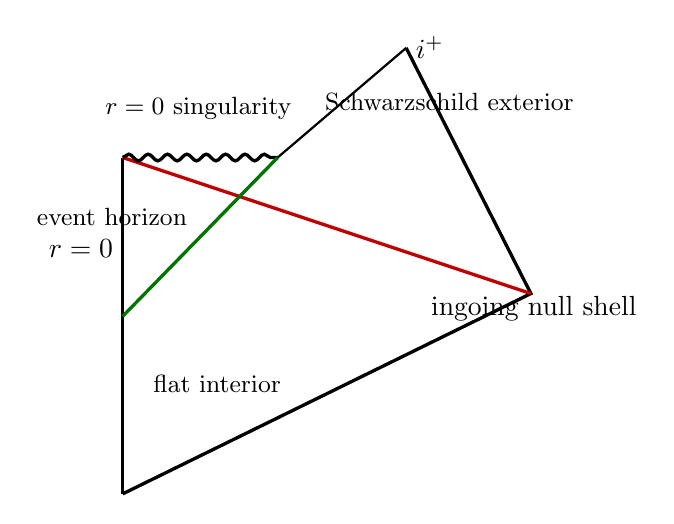
\begin{tikzpicture}[scale=0.96]
\coordinate (A) at (0,-2.8);
\coordinate (B) at (0,1.65);
\coordinate (C) at (2.05,1.65);
\coordinate (D) at (5.4,-0.15);
\coordinate (E) at (3.75,3.10);
\coordinate (H0) at (0,-0.45);
\draw[very thick] (A)--(B);
\draw[very thick] (A)--(D)--(E);
\draw[very thick,red!75!black] (D)--(B);
\draw[very thick,decorate,decoration={snake,amplitude=1.2pt,segment length=7pt}] (B)--(C);
\draw[very thick,green!45!black] (H0)--(C);
\draw[thick] (C)--(E);
\node[left] at (0,0.45) {\(r=0\)};
\node[below right] at (3.95,-0.05) {ingoing null shell};
\node[font=\small] at (1.25,-1.35) {flat interior};
\node[font=\small,anchor=west] at (2.55,2.38) {Schwarzschild exterior};
\node[above,font=\small] at (1.0,2.02) {\(r=0\) singularity};
\node[above left,font=\small] at (0.98,0.62) {event horizon};
\node[right] at (E) {\(i^+\)};
\end{tikzpicture}
\caption{La geometría del colapso. La capa roja une un interior plano con un exterior de Schwarzschild. El horizonte de sucesos verde comienza antes, en la región plana, y termina en la frontera futura de la región del agujero negro.}
\label{fig:l05-collapse}
\end{figure}

Esta construcción responde a una pregunta que dejaba abierta la solución eterna. Un agujero negro formado por colapso no tiene un agujero blanco pasado ni un segundo universo asintótico. Aun así, tiene una singularidad futura.

\section{El horizonte es una frontera global}

La antigua condición \(r=2GM\) identificaba el horizonte en la geometría estacionaria de Schwarzschild, pero no es la definición que necesitamos en un espacio-tiempo dinámico.

\begin{definition}
El horizonte de sucesos futuro es la frontera del conjunto de sucesos desde los cuales se puede enviar una señal causal dirigida al futuro hasta el infinito nulo futuro.
\end{definition}

En el diagrama de colapso, sigamos el rayo nulo saliente que está justo al límite de no poder escapar. Los rayos apenas por fuera llegan al infinito; los apenas por dentro terminan en la singularidad. Esa superficie separadora es el horizonte verdadero.

\begin{figure}[htbp]
\centering
\includegraphics[width=0.72\textwidth]{lecture_05_figure_06.png}
\caption{La construcción completa en la pizarra. La capa entrante es roja y el horizonte de sucesos, verde; parte de la línea verde se encuentra en la región todavía plana, por debajo de la capa.}
\lectureframe{00:39:10.000}
\end{figure}

Ahora resulta imposible pasar por alto la característica sorprendente. El horizonte se prolonga hacia atrás, hasta una región a la que la capa aún no ha llegado. Allí la geometría es localmente plana, y un observador que atraviese esa línea no detecta ningún pulso de curvatura, pared ni destello. Sin embargo, ya no puede llegar al infinito, porque la capa futura cerrará todas las rutas de escape posibles. Los horizontes de sucesos son teleológicos precisamente en este sentido global: para localizar uno hace falta conocer el futuro completo del espacio-tiempo.\editorialnote{Ningún experimento local puede determinar que se acaba de cruzar un horizonte de sucesos liso. Otras nociones, como los horizontes aparentes o atrapantes, son más locales y durante el colapso no tienen por qué coincidir con el horizonte de sucesos.}

La analogía del desagüe permite aislar la idea causal. Imaginemos a una persona remando cerca de un desagüe tapado en un lago en calma. Si el tapón permaneciera allí para siempre, podría alejarse. Pero si se sabe con certeza que alguien lo va a quitar, la corriente posterior podría impedirle escapar aunque todavía no se mueva el agua. Una catarata del Niágara congelada ilustra lo mismo: que el agua esté en calma no garantiza que haya una ruta segura en el futuro.

\begin{classroomqa}
\audiencequestion{¿Se quita el tapón porque la capa esférica de luz se concentra cada vez más?\lecturetimestamp{00:43:13}}
\lecturerresponse{La concentración es lo que crea el agujero negro, pero la analogía del desagüe tiene un propósito más acotado: ya se puede haber cruzado el punto de no retorno antes de que ocurra nada dramático en el entorno local.}
\end{classroomqa}

\subsection{Un horizonte formado por esferas crecientes}

Cada punto del horizonte en el diagrama reducido representa una \(S^2\). En el primer punto del horizonte, esa esfera tiene área nula. Al avanzar hacia arriba a lo largo del horizonte, la esfera crece hasta que su radio areal alcanza
\begin{equation}
R_s=\frac{2GM}{c^2}.
\end{equation}
En un agujero estacionario permanece de ese tamaño, y vuelve a crecer si cae más energía.

\editorialnote{En el diagrama idealizado de colapso esférico, los generadores del horizonte se encuentran en un punto de formación, o pliegue, en \(r=0\). Es esa esfera límite la que tiene área nula; no debe interpretarse que un horizonte de Schwarzschild finito se contraiga de repente hasta un punto.}

\subsection{Qué puede reconstruir el observador distante}

La larga discusión que sigue distingue entre el observador que ya está dentro del horizonte global y la historia que lo llevó allí.

\begin{classroomqa}
\audiencequestion{¿Cuál es la situación de la persona atrapada antes de que llegue la capa? Desde el punto de vista del observador distante, ¿está fuera del horizonte?\lecturetimestamp{00:44:03}}
\lecturerresponse{No. Una vez que la línea de universo queda detrás del horizonte de sucesos, su futuro alcanza la singularidad y ninguna señal nueva procedente de esa persona llega al observador distante. Sin embargo, esa persona no empezó a existir allí. Partículas anteriores, antepasados u otra energía precursora entraron desde una región visible.}
\end{classroomqa}

Por tanto, el observador distante puede ver cómo la materia precursora se acerca al horizonte sin recibir jamás una señal desde el otro lado. No hay contradicción en ver a través de la capa entrante: está hecha de luz, y el observador también puede verla y deducir que se ha formado un agujero negro.

\begin{classroomqa}
\audiencequestion{¿La línea de visión atraviesa la capa en colapso, y puede el observador exterior saber aun así que se formó el agujero?\lecturetimestamp{00:46:51}}
\lecturerresponse{Sí. El observador ve la capa entrante y puede recibir luz cuya trayectoria la atraviesa mientras todavía es capaz de escapar. Lo extraño es que la materia precursora se acerca al horizonte recién determinado incluso antes de que la capa llegue al centro.}
\end{classroomqa}

\begin{classroomqa}
\audiencequestion{¿Continúa esto la regla según la cual, desde el exterior, parece que la materia se comprime sobre el horizonte?\lecturetimestamp{00:47:49}}
\lecturerresponse{Sí. En la descripción exterior, la materia sigue asociada al horizonte y sufre un corrimiento al rojo cada vez mayor, hasta que el posterior proceso cuántico de evaporación del agujero negro cambia la situación.}
\end{classroomqa}

Esta descripción exterior da pie al siguiente tema. Si la información parece quedar adherida a una superficie bidimensional, resulta menos sorprendente que la entropía de un agujero negro sea proporcional al área de esa superficie.

\section{Entropía y temperatura observada desde el infinito}

Cerca de un horizonte grande podemos aproximar la superficie esférica por un plano local, igual que usamos la aproximación de Tierra plana en un laboratorio pequeño. Reunimos entonces dos hechos de la discusión anterior:
\begin{equation}
\begin{aligned}
S_{\mathrm{BH}}&\propto A_H,\\
\Delta A_H&\sim \ell_P^2
\quad\text{per added bit, schematically}.
\end{aligned}
\end{equation}
La regla mnemotécnica de un bit por área de Planck expresa la ley de área; no constituye una derivación microscópica.

La temperatura de Hawking de un agujero negro de Schwarzschild, medida lejos de él, es
\begin{equation}
T_H=\frac{\hbar c^3}{8\pi GMk_B}.
\label{eq:l05-hawking}
\end{equation}
Con \(R_s=2GM/c^2\),
\begin{equation}
T_H=\frac{\hbar c}{4\pi k_B R_s}.
\label{eq:l05-hawking-radius}
\end{equation}
Así, los agujeros más grandes son más fríos.

\begin{classroomqa}
\audiencequestion{¿Puede depender la temperatura de la posición?\lecturetimestamp{00:52:43}}
\lecturerresponse{En una conversación corriente, es evidente que sí: Nueva York y Stanford no tienen por qué estar a la misma temperatura. La pregunta más precisa se refiere a un sistema en equilibrio térmico gravitatorio. En ese caso, las lecturas de los termómetros locales pueden variar con la altura aunque la temperatura de equilibrio corregida por el corrimiento gravitatorio sea constante.}
\end{classroomqa}

La temperatura se mide mediante las energías cinéticas locales. En una atmósfera tenue sobre una Tierra caliente, las moléculas pierden energía cinética al ascender y la ganan al descender. Los fotones sufren un corrimiento al rojo al subir y al azul al bajar. Por tanto, un termómetro situado abajo y otro situado arriba no tienen por qué indicar la misma escala local de energía.

En un espacio-tiempo estático, la relación de equilibrio es
\begin{equation}
T_{\mathrm{loc}}(r)\sqrt{-g_{tt}(r)}=T_\infty,
\label{eq:l05-tolman}
\end{equation}
la ley de Tolman. La temperatura de Hawking de la ecuación~\eqref{eq:l05-hawking} es \(T_\infty\), el valor normalizado en el infinito.

\section{La atmósfera estática caliente cerca del horizonte}

Sea \(\rho\) la distancia propia hacia afuera desde el horizonte. Cerca de un horizonte de Schwarzschild grande, la ecuación~\eqref{eq:l05-tolman} se convierte en
\begin{equation}
k_B T_{\mathrm{loc}}(\rho)
\simeq\frac{\hbar c}{2\pi\rho},
\label{eq:l05-local-temperature-si}
\end{equation}
o, en unidades \(c=\hbar=k_B=1\),
\begin{equation}
T_{\mathrm{loc}}(\rho)=\frac{1}{2\pi\rho}.
\label{eq:l05-local-temperature}
\end{equation}

\begin{figure}[htbp]
\centering
\includegraphics[width=0.72\textwidth]{lecture_05_figure_07.png}
\caption{La temperatura de Hawking asintótica y la temperatura local cerca del horizonte \(T(\rho)=1/(2\pi\rho)\) que aparece en la pizarra.}
\lectureframe{01:02:40.000}
\end{figure}

Un termómetro diminuto suspendido de un cable a distancia fija \(\rho\) indica una temperatura cada vez mayor a medida que se baja. Un átomo mantenido en esa atmósfera estática se excita, luego se ioniza y después se disocia; a energías locales aún mayores, incluso los núcleos y los hadrones dejan de mantenerse intactos. Al bajar a una persona con los pies por delante, se obtiene un diagnóstico memorable: un pie caliente.

La palabra \emph{mantenido} es esencial. Esta divergencia corresponde a un detector que se mantiene estacionario mediante aceleración. Describe la atmósfera térmica con el corrimiento gravitatorio respecto al tiempo exterior. Un detector en caída libre sigue otra trayectoria y, para un agujero suficientemente grande en un estado cuántico regular, no tiene por qué encontrar un baño divergente en el horizonte.\editorialnote{Esta distinción separa las temperaturas de Tolman y de aceleración que observan los observadores estáticos de la experiencia local regular de un observador en caída libre. La clase convierte deliberadamente ese contraste en un problema operacional, en lugar de resolverlo solo mediante la terminología.}

El umbral de ionización concreta el conflicto.

\begin{classroomqa}
\audiencequestion{¿Cuánta energía hace falta para ionizar el hidrógeno?\lecturetimestamp{01:06:53}}
\lecturerresponse{La clase responde \(13\) electronvoltios e identifica correctamente la energía de ionización del estado fundamental, que es \(13.6\,\mathrm{eV}\). La estimación acompañante de unos pocos miles de kelvin es demasiado baja, pero para el argumento solo hace falta que exista un umbral finito.}
\end{classroomqa}

En efecto,
\begin{equation}
\frac{13.6\,\mathrm{eV}}{k_B}\simeq1.58\times10^5\,\mathrm{K}.
\end{equation}
Por tanto, hay una distancia propia pequeña \(\rho_{\mathrm{ion}}\) a la que la temperatura estática alcanza la escala de ionización. Una extrapolación estática indica que el átomo ya debería estar ionizado allí, fuera del horizonte. En cambio, un átomo en caída libre no espera encontrar una pared local y puede cruzar el horizonte en un tiempo propio finito. ¿Puede un observador exterior realizar un experimento que permita decidir entre estas descripciones?

\section{Un microscopio de Heisenberg}

Antes de aplicar la pregunta a un agujero negro, recordemos el microscopio de fotones. Para localizar una partícula con resolución \(\Delta x\), la longitud de onda de la sonda debe satisfacer
\begin{equation}
\lambda\lesssim\Delta x.
\end{equation}
Así, un fotón transporta un momento de al menos
\begin{equation}
p_\gamma\gtrsim\frac{\hbar}{\Delta x}.
\label{eq:l05-microscope}
\end{equation}
La dispersión de ese fotón produce un retroceso del mismo orden. Si primero se mide la posición y enseguida se comprueba la velocidad, la segunda medición observa un estado que la primera ya ha cambiado. El experimento produce la condición que pretendía descartar.

\begin{figure}[htbp]
\centering
\includegraphics[width=0.70\textwidth]{lecture_05_figure_08.png}
\caption{Estimaciones del microscopio para \(\Delta x\gtrsim\lambda\) y \(p_\gamma\gtrsim\hbar/\Delta x\).}
\lectureframe{01:11:50.000}
\end{figure}

No se trata simplemente de una limitación de la óptica clásica. Las ondas clásicas se podrían hacer arbitrariamente débiles; la mecánica cuántica exige al menos un cuanto para que se produzca un evento de detección. Por tanto, mejorar la resolución espacial requiere una transferencia de momento finita.

\section{El experimento cerca del horizonte}

Ahora supongamos que un átomo cae a través de la capa que comienza en \(\rho_{\mathrm{ion}}\). Respecto al marco estático, se mueve hacia adentro a una velocidad cercana a \(c\), de modo que el intervalo disponible antes de cruzar el horizonte es del orden de
\begin{equation}
\Delta\tau\sim\frac{\rho_{\mathrm{ion}}}{c}.
\label{eq:l05-fall-time}
\end{equation}
Después de cruzarlo, no se puede enviar ningún resultado al exterior. La medición debe distinguir entre un átomo intacto y uno ionizado durante ese breve intervalo.

Para resolver el átomo dentro de la capa se requiere
\begin{equation}
\lambda\lesssim\rho_{\mathrm{ion}}.
\end{equation}
Por consiguiente, la energía de la sonda está limitada por
\begin{equation}
E_\gamma=cp_\gamma
\gtrsim\frac{\hbar c}{\rho_{\mathrm{ion}}}.
\label{eq:l05-probe-energy}
\end{equation}
Salvo por el factor \(2\pi\), esta es la misma escala que en la ecuación~\eqref{eq:l05-local-temperature-si}:
\begin{equation}
E_\gamma\gtrsim2\pi k_B T_{\mathrm{loc}}(\rho_{\mathrm{ion}}).
\label{eq:l05-probe-temperature}
\end{equation}
El fotón con energía suficiente para resolver el evento también tiene energía suficiente para ionizar el átomo.

\begin{figure}[htbp]
\centering
\includegraphics[width=0.72\textwidth]{lecture_05_figure_09.png}
\caption{La estimación cerca del horizonte en la pizarra: \(\lambda<\rho\) exige una energía local de la sonda del orden de \(\hbar c/\rho\).}
\lectureframe{01:18:30.000}
\end{figure}

\begin{classroomqa}
\audiencequestion{¿Ese fotón de alta energía ionizaría el átomo incluso en su marco de caída libre?\lecturetimestamp{01:19:07}}
\lecturerresponse{Sí. El átomo recibe el impacto de un cuanto real de alta energía y retrocede o se ioniza en su propio marco local. La medición no revela una caída sin perturbar, sino que la sustituye por una caída perturbada.}
\end{classroomqa}

\begin{classroomqa}
\audiencequestion{¿Y si el átomo simplemente cae y nadie realiza el experimento?\lecturetimestamp{01:19:39}}
\lecturerresponse{Entonces no se produce esta perturbación en particular. Si un observador exterior sí realiza el experimento de alta resolución, el átomo corre peligro. El argumento se refiere a lo que puede verificarse desde el exterior, no demuestra que un objeto que cae sin ser medido se queme.}
\end{classroomqa}

\subsection{¿Podría funcionar mejor un termómetro o un transmisor?}

Mover el aparato no resuelve el problema de la información.

\begin{classroomqa}
\audiencequestion{¿Se podría medir más lejos, deducir el gradiente o dejar que un termómetro en caída libre registre la temperatura y recuperarlo después?\lecturetimestamp{01:19:51}}
\lecturerresponse{Para conocer el registro cerca del horizonte, algo debe interactuar con el termómetro y devolver información en forma de cuantos. Dar la vuelta al termómetro requiere una aceleración violenta, mientras que leerlo a distancia requiere emisión o dispersión. Cualquiera de las dos opciones cambia el sistema físico cuya historia sin perturbar se pretendía comprobar.}
\end{classroomqa}

\begin{classroomqa}
\audiencequestion{¿La alta energía de la sonda necesaria para lograr una resolución pequeña es el mismo problema que conseguir que la observación reflejada salga de la región cercana al horizonte?\lecturetimestamp{01:21:51}}
\lecturerresponse{Son dos aspectos de la misma escala afectada por el corrimiento gravitatorio. El fotón puede tener poca energía cuando finalmente llega al infinito, porque pierde energía al ascender, pero donde resuelve el átomo debe tener una frecuencia local alta.}
\end{classroomqa}

\editorialnote{Un fotón emitido justo fuera del horizonte no tiene por qué poseer mucha energía para escapar. Lo decisivo aquí es que codifique el suceso dentro de un tiempo propio y una distancia del orden de \(\rho\); el corrimiento gravitatorio al rojo relaciona esa frecuencia local alta con una frecuencia asintótica mucho menor.}

\begin{classroomqa}
\audiencequestion{¿Podría el propio objeto emitir la información en lugar de recibir el impacto de un fotón externo?\lecturetimestamp{01:22:51}}
\lecturerresponse{Sí, pero la emisión local sigue necesitando el ancho de banda requerido para identificar lo que ocurrió durante el breve intervalo. Además, la emisión hace retroceder al objeto. Sustituir la luz reflejada por un transmisor no permite obtener un registro sin costo físico.}
\end{classroomqa}

\begin{classroomqa}
\audiencequestion{El átomo que cae tiene una dirección preferente. ¿Se está llamando temperatura a su energía cinética dirigida?\lecturetimestamp{01:23:10}}
\lecturerresponse{No. Lanzar una pelota de béisbol no la calienta. La energía de la caída colectiva y la agitación térmica son distintas. La temperatura del argumento corresponde a la atmósfera estática de radiación que lo rodea, no al movimiento del centro de masas del átomo.}
\end{classroomqa}

\begin{classroomqa}
\audiencequestion{¿Podría un laboratorio que cae junto con el átomo usar un campo magnético para comprobar si está ionizado?\lecturetimestamp{01:23:50}}
\lecturerresponse{Un laboratorio puede realizar una prueba local. La dificultad consiste en comunicar el resultado al exterior antes de cruzar el horizonte. Esa comunicación vuelve a requerir una interacción y cuantos salientes con la resolución local necesaria.}
\end{classroomqa}

\begin{classroomqa}
\audiencequestion{¿El transmisor incorporado al termómetro necesitaría tanta energía local que destruiría el aparato?\lecturetimestamp{01:24:57}}
\lecturerresponse{Esa es la misma limitación expresada en términos de ingeniería. Lo bastante cerca del horizonte, la energía de la señal requerida en la escala local pertinente es comparable a la escala térmica que se pretende medir.}
\end{classroomqa}

\begin{classroomqa}
\audiencequestion{¿Es tan estrecha la región de alta temperatura que no hay tiempo para hacer la medición con calma?\lecturetimestamp{01:25:15}}
\lecturerresponse{Exactamente. Su espesor propio es del orden de \(\rho\), y el tiempo de cruce es del orden de \(\rho/c\). Puede describirse la limitación como resolución espacial o como ancho de banda temporal; cualquiera de las dos descripciones exige un momento o una energía local elevados.}
\end{classroomqa}

La estimación correspondiente para el producto tiempo-ancho de banda es
\begin{equation}
\Delta E\,\Delta\tau\gtrsim\hbar.
\end{equation}
Aquí debe entenderse como una cota de resolución de Fourier u operacional, no como una relación de incertidumbre entre operadores con el mismo estatus que \(\Delta x\,\Delta p\geq\hbar/2\). La conferencia recurre heurísticamente a la incertidumbre tiempo-energía; la ecuación~\eqref{eq:l05-probe-energy}, derivada de la resolución espacial, es la parte más sólida del argumento.

\begin{classroomqa}
\audiencequestion{¿Se podrían usar sondas de menor energía y menor resolución en muchos átomos y obtener la respuesta mediante métodos estadísticos?\lecturetimestamp{01:26:26}}
\lecturerresponse{Es una pregunta razonable, que queda abierta en clase. Cada átomo solo atraviesa la región una vez, y cualquier señal recuperada aún debe contener información suficiente para identificar el breve suceso cercano al horizonte. La conferencia apela al principio de incertidumbre, pero no ofrece una demostración completa de imposibilidad estadística.}
\end{classroomqa}

\enlargethispage{2\baselineskip}
\section{Lo que se ha establecido y lo que no}

El argumento no predice que una persona en caída libre tenga que sentir la temperatura estática divergente.

\begin{classroomqa}
\audiencequestion{¿Estamos diciendo que podemos predecir que la persona que cae no sentirá la temperatura?\lecturetimestamp{01:27:38}}
\lecturerresponse{No. El resultado es más limitado: un experimento exterior diseñado para confirmar que el átomo no experimentó la perturbación de alta temperatura genera una perturbación de la misma escala. Eso es todo lo que establece este análisis operacional.}
\end{classroomqa}

Así pues, la conclusión no es un teorema del cortafuegos, ni una demostración de que quien cae se quema, ni una demostración de que no ocurre nada. Es un límite a la verificación desde el exterior: \emph{resolver el suceso no perturbado cercano al horizonte requiere una sonda que lo perturbe}.
Si se realiza el experimento, sus cuantos producen el efecto que se pretendía comprobar. Si no se realiza, este argumento por sí solo no atribuye ningún otro hecho accesible experimentalmente. La comparación con el experimento de la doble rendija es deliberada: preguntar por cuál rendija pasó la partícula sin medir su trayectoria y preguntar qué certifica un aparato exterior sin que haya interacción son, en ambos casos, intentos de dar una respuesta operacional cuando no es posible obtener la evidencia propuesta.
